% Options for packages loaded elsewhere
\PassOptionsToPackage{unicode}{hyperref}
\PassOptionsToPackage{hyphens}{url}
%
\documentclass[
]{article}
\usepackage{amsmath,amssymb}
\usepackage{lmodern}
\usepackage{ifxetex,ifluatex}
\ifnum 0\ifxetex 1\fi\ifluatex 1\fi=0 % if pdftex
  \usepackage[T1]{fontenc}
  \usepackage[utf8]{inputenc}
  \usepackage{textcomp} % provide euro and other symbols
\else % if luatex or xetex
  \usepackage{unicode-math}
  \defaultfontfeatures{Scale=MatchLowercase}
  \defaultfontfeatures[\rmfamily]{Ligatures=TeX,Scale=1}
\fi
% Use upquote if available, for straight quotes in verbatim environments
\IfFileExists{upquote.sty}{\usepackage{upquote}}{}
\IfFileExists{microtype.sty}{% use microtype if available
  \usepackage[]{microtype}
  \UseMicrotypeSet[protrusion]{basicmath} % disable protrusion for tt fonts
}{}
\makeatletter
\@ifundefined{KOMAClassName}{% if non-KOMA class
  \IfFileExists{parskip.sty}{%
    \usepackage{parskip}
  }{% else
    \setlength{\parindent}{0pt}
    \setlength{\parskip}{6pt plus 2pt minus 1pt}}
}{% if KOMA class
  \KOMAoptions{parskip=half}}
\makeatother
\usepackage{xcolor}
\IfFileExists{xurl.sty}{\usepackage{xurl}}{} % add URL line breaks if available
\IfFileExists{bookmark.sty}{\usepackage{bookmark}}{\usepackage{hyperref}}
\hypersetup{
  pdftitle={Bellabeat Product Analysis},
  pdfauthor={Pritee Kadam},
  hidelinks,
  pdfcreator={LaTeX via pandoc}}
\urlstyle{same} % disable monospaced font for URLs
\usepackage[margin=1in]{geometry}
\usepackage{color}
\usepackage{fancyvrb}
\newcommand{\VerbBar}{|}
\newcommand{\VERB}{\Verb[commandchars=\\\{\}]}
\DefineVerbatimEnvironment{Highlighting}{Verbatim}{commandchars=\\\{\}}
% Add ',fontsize=\small' for more characters per line
\usepackage{framed}
\definecolor{shadecolor}{RGB}{248,248,248}
\newenvironment{Shaded}{\begin{snugshade}}{\end{snugshade}}
\newcommand{\AlertTok}[1]{\textcolor[rgb]{0.94,0.16,0.16}{#1}}
\newcommand{\AnnotationTok}[1]{\textcolor[rgb]{0.56,0.35,0.01}{\textbf{\textit{#1}}}}
\newcommand{\AttributeTok}[1]{\textcolor[rgb]{0.77,0.63,0.00}{#1}}
\newcommand{\BaseNTok}[1]{\textcolor[rgb]{0.00,0.00,0.81}{#1}}
\newcommand{\BuiltInTok}[1]{#1}
\newcommand{\CharTok}[1]{\textcolor[rgb]{0.31,0.60,0.02}{#1}}
\newcommand{\CommentTok}[1]{\textcolor[rgb]{0.56,0.35,0.01}{\textit{#1}}}
\newcommand{\CommentVarTok}[1]{\textcolor[rgb]{0.56,0.35,0.01}{\textbf{\textit{#1}}}}
\newcommand{\ConstantTok}[1]{\textcolor[rgb]{0.00,0.00,0.00}{#1}}
\newcommand{\ControlFlowTok}[1]{\textcolor[rgb]{0.13,0.29,0.53}{\textbf{#1}}}
\newcommand{\DataTypeTok}[1]{\textcolor[rgb]{0.13,0.29,0.53}{#1}}
\newcommand{\DecValTok}[1]{\textcolor[rgb]{0.00,0.00,0.81}{#1}}
\newcommand{\DocumentationTok}[1]{\textcolor[rgb]{0.56,0.35,0.01}{\textbf{\textit{#1}}}}
\newcommand{\ErrorTok}[1]{\textcolor[rgb]{0.64,0.00,0.00}{\textbf{#1}}}
\newcommand{\ExtensionTok}[1]{#1}
\newcommand{\FloatTok}[1]{\textcolor[rgb]{0.00,0.00,0.81}{#1}}
\newcommand{\FunctionTok}[1]{\textcolor[rgb]{0.00,0.00,0.00}{#1}}
\newcommand{\ImportTok}[1]{#1}
\newcommand{\InformationTok}[1]{\textcolor[rgb]{0.56,0.35,0.01}{\textbf{\textit{#1}}}}
\newcommand{\KeywordTok}[1]{\textcolor[rgb]{0.13,0.29,0.53}{\textbf{#1}}}
\newcommand{\NormalTok}[1]{#1}
\newcommand{\OperatorTok}[1]{\textcolor[rgb]{0.81,0.36,0.00}{\textbf{#1}}}
\newcommand{\OtherTok}[1]{\textcolor[rgb]{0.56,0.35,0.01}{#1}}
\newcommand{\PreprocessorTok}[1]{\textcolor[rgb]{0.56,0.35,0.01}{\textit{#1}}}
\newcommand{\RegionMarkerTok}[1]{#1}
\newcommand{\SpecialCharTok}[1]{\textcolor[rgb]{0.00,0.00,0.00}{#1}}
\newcommand{\SpecialStringTok}[1]{\textcolor[rgb]{0.31,0.60,0.02}{#1}}
\newcommand{\StringTok}[1]{\textcolor[rgb]{0.31,0.60,0.02}{#1}}
\newcommand{\VariableTok}[1]{\textcolor[rgb]{0.00,0.00,0.00}{#1}}
\newcommand{\VerbatimStringTok}[1]{\textcolor[rgb]{0.31,0.60,0.02}{#1}}
\newcommand{\WarningTok}[1]{\textcolor[rgb]{0.56,0.35,0.01}{\textbf{\textit{#1}}}}
\usepackage{graphicx}
\makeatletter
\def\maxwidth{\ifdim\Gin@nat@width>\linewidth\linewidth\else\Gin@nat@width\fi}
\def\maxheight{\ifdim\Gin@nat@height>\textheight\textheight\else\Gin@nat@height\fi}
\makeatother
% Scale images if necessary, so that they will not overflow the page
% margins by default, and it is still possible to overwrite the defaults
% using explicit options in \includegraphics[width, height, ...]{}
\setkeys{Gin}{width=\maxwidth,height=\maxheight,keepaspectratio}
% Set default figure placement to htbp
\makeatletter
\def\fps@figure{htbp}
\makeatother
\setlength{\emergencystretch}{3em} % prevent overfull lines
\providecommand{\tightlist}{%
  \setlength{\itemsep}{0pt}\setlength{\parskip}{0pt}}
\setcounter{secnumdepth}{-\maxdimen} % remove section numbering
\usepackage{booktabs}
\usepackage{longtable}
\usepackage{array}
\usepackage{multirow}
\usepackage{wrapfig}
\usepackage{float}
\usepackage{colortbl}
\usepackage{pdflscape}
\usepackage{tabu}
\usepackage{threeparttable}
\usepackage{threeparttablex}
\usepackage[normalem]{ulem}
\usepackage{makecell}
\usepackage{xcolor}
\ifluatex
  \usepackage{selnolig}  % disable illegal ligatures
\fi

\title{Bellabeat Product Analysis}
\author{Pritee Kadam}
\date{9/28/2021}

\begin{document}
\maketitle

\hypertarget{bellabeat-products-analysis}{%
\section{Bellabeat Products
Analysis}\label{bellabeat-products-analysis}}

\hypertarget{the-problem-statement}{%
\subsection{The problem statement}\label{the-problem-statement}}

``Bellabeat, a high-tech manufacturer of health-focused products for
women. Bellabeat wants to expand their business for one of their
products so they wants to analyse the usage of one of their products in
order to gain insight into how people are already using their smart
devices.Then, using this information,she(Urška Sršen, cofounder and
Chief Creative Officer of Bellabeat) would like high-level
recommendations for how these trends can inform Bellabeat marketing
strategy''

\hypertarget{key-stakeholders-}{%
\subsubsection{Key stakeholders:-}\label{key-stakeholders-}}

Urška Sršen: Bellabeat's co-founder and Chief Creative Officer Sando
Mur: Mathematician and Bellabeat's co-founder Bellabeat marketing
analytics team

\hypertarget{introduction-}{%
\subsubsection{Introduction:-}\label{introduction-}}

This is a capstone project for my Google Data Analytics Capstone. In
this case study, I will be analyzing one of Bellabeat's smart device
data to gain insight into how consumers are using their smart devices,
Bellabeat is a high-tech manufacturer of health focused products for
women. The insights I discover will then help guide to decide or enhance
marketing strategy for the company

\hypertarget{ask-}{%
\subsubsection{1) Ask:-}\label{ask-}}

\begin{itemize}
\tightlist
\item
  Key Objectives:
\end{itemize}

\begin{enumerate}
\def\labelenumi{\arabic{enumi}.}
\tightlist
\item
  What are some daily habit trends in smart devise usage?
\item
  How could these daily habit trends apply to Bellabeat customers?
\item
  How could these daily habit trends help influence the Bellabeat
  marketing strategy?
\end{enumerate}

\hypertarget{prepare-}{%
\subsubsection{2) Prepare:-}\label{prepare-}}

\begin{verbatim}
Data preparation:

 Source, Licensing, Privacy
\end{verbatim}

Source: FitBit Fitness Tracker Data - (Dataset made available through
Mobius)

License: CC0: Public Domain

Privacy: This Kaggle data set contains personal fitness tracker from
30\\
Fitbit users who consented to the submission of personal tracker
data,including minute-level output for physical activity, heart rate,
and sleep monitoring. It includes information about daily activity,
steps, and heart rate that can be used to explore users' habits.

\hypertarget{process}{%
\subsubsection{3) Process:}\label{process}}

\hypertarget{importing-necessory-packages}{%
\paragraph{importing necessory
packages}\label{importing-necessory-packages}}

\begin{Shaded}
\begin{Highlighting}[]
 \ControlFlowTok{if}\NormalTok{ (}\SpecialCharTok{!}\FunctionTok{require}\NormalTok{(}\StringTok{\textquotesingle{}tidyverse\textquotesingle{}}\NormalTok{))}
\NormalTok{ \{}
  \FunctionTok{install.packages}\NormalTok{(}\StringTok{\textquotesingle{}tidyverse\textquotesingle{}}\NormalTok{);}
   \FunctionTok{library}\NormalTok{(tidyverse);}
\NormalTok{ \}}
\end{Highlighting}
\end{Shaded}

\begin{verbatim}
## Loading required package: tidyverse
\end{verbatim}

\begin{verbatim}
## -- Attaching packages --------------------------------------- tidyverse 1.3.1 --
\end{verbatim}

\begin{verbatim}
## v ggplot2 3.3.5     v purrr   0.3.4
## v tibble  3.1.4     v dplyr   1.0.7
## v tidyr   1.1.3     v stringr 1.4.0
## v readr   2.0.1     v forcats 0.5.1
\end{verbatim}

\begin{verbatim}
## -- Conflicts ------------------------------------------ tidyverse_conflicts() --
## x dplyr::filter() masks stats::filter()
## x dplyr::lag()    masks stats::lag()
\end{verbatim}

\begin{Shaded}
\begin{Highlighting}[]
\ControlFlowTok{if}\NormalTok{(}\SpecialCharTok{!}\FunctionTok{require}\NormalTok{(}\StringTok{\textquotesingle{}tidyverse\textquotesingle{}}\NormalTok{))}
\NormalTok{\{}
  \FunctionTok{install.packages}\NormalTok{(}\StringTok{\textquotesingle{}here\textquotesingle{}}\NormalTok{);}
  \FunctionTok{library}\NormalTok{(here);}
\NormalTok{\}}
\end{Highlighting}
\end{Shaded}

\begin{Shaded}
\begin{Highlighting}[]
\ControlFlowTok{if}\NormalTok{(}\SpecialCharTok{!}\FunctionTok{require}\NormalTok{(}\StringTok{\textquotesingle{}skimr\textquotesingle{}}\NormalTok{))}
\NormalTok{\{}
  \FunctionTok{install.packages}\NormalTok{(}\StringTok{\textquotesingle{}skimr\textquotesingle{}}\NormalTok{);}
  \FunctionTok{library}\NormalTok{(skimr);}
\NormalTok{\}}
\end{Highlighting}
\end{Shaded}

\begin{verbatim}
## Loading required package: skimr
\end{verbatim}

\begin{Shaded}
\begin{Highlighting}[]
\ControlFlowTok{if}\NormalTok{(}\SpecialCharTok{!}\FunctionTok{require}\NormalTok{(}\StringTok{\textquotesingle{}janitor\textquotesingle{}}\NormalTok{))}
\NormalTok{\{}
  \FunctionTok{install.packages}\NormalTok{(}\StringTok{\textquotesingle{}janitor\textquotesingle{}}\NormalTok{);}
  \FunctionTok{library}\NormalTok{(janitor)}
\NormalTok{\} }
\end{Highlighting}
\end{Shaded}

\begin{verbatim}
## Loading required package: janitor
\end{verbatim}

\begin{verbatim}
## 
## Attaching package: 'janitor'
\end{verbatim}

\begin{verbatim}
## The following objects are masked from 'package:stats':
## 
##     chisq.test, fisher.test
\end{verbatim}

\begin{Shaded}
\begin{Highlighting}[]
\ControlFlowTok{if}\NormalTok{(}\SpecialCharTok{!}\FunctionTok{require}\NormalTok{(}\StringTok{\textquotesingle{}lubridate\textquotesingle{}}\NormalTok{))}
\NormalTok{\{}
\FunctionTok{install.packages}\NormalTok{(}\StringTok{\textquotesingle{}lubridate\textquotesingle{}}\NormalTok{);}
  \FunctionTok{library}\NormalTok{(lubridate)}
\NormalTok{\}  }
\end{Highlighting}
\end{Shaded}

\begin{verbatim}
## Loading required package: lubridate
\end{verbatim}

\begin{verbatim}
## 
## Attaching package: 'lubridate'
\end{verbatim}

\begin{verbatim}
## The following objects are masked from 'package:base':
## 
##     date, intersect, setdiff, union
\end{verbatim}

\begin{Shaded}
\begin{Highlighting}[]
\ControlFlowTok{if}\NormalTok{(}\SpecialCharTok{!}\FunctionTok{require}\NormalTok{(}\StringTok{\textquotesingle{}dplyr\textquotesingle{}}\NormalTok{))}
\NormalTok{\{}
\FunctionTok{install.packages}\NormalTok{(}\StringTok{\textquotesingle{}dplyr\textquotesingle{}}\NormalTok{);}
  \FunctionTok{library}\NormalTok{(dplyr);}
\NormalTok{\}}
\end{Highlighting}
\end{Shaded}

\begin{Shaded}
\begin{Highlighting}[]
\ControlFlowTok{if}\NormalTok{(}\SpecialCharTok{!}\FunctionTok{require}\NormalTok{(}\StringTok{\textquotesingle{}ggplot2\textquotesingle{}}\NormalTok{))}
\NormalTok{\{}
\FunctionTok{install.packages}\NormalTok{(}\StringTok{\textquotesingle{}ggplot2\textquotesingle{}}\NormalTok{);}
  \FunctionTok{library}\NormalTok{(ggplot2);}
\NormalTok{\}}
\end{Highlighting}
\end{Shaded}

\begin{Shaded}
\begin{Highlighting}[]
\ControlFlowTok{if}\NormalTok{(}\SpecialCharTok{!}\FunctionTok{require}\NormalTok{(}\StringTok{\textquotesingle{}tidyr\textquotesingle{}}\NormalTok{))}
\NormalTok{\{}
  \FunctionTok{install.packages}\NormalTok{(}\StringTok{\textquotesingle{}tidyr\textquotesingle{}}\NormalTok{);}
  \FunctionTok{library}\NormalTok{(tidyr);}
\NormalTok{\}  }
\end{Highlighting}
\end{Shaded}

\begin{Shaded}
\begin{Highlighting}[]
\ControlFlowTok{if}\NormalTok{(}\SpecialCharTok{!}\FunctionTok{require}\NormalTok{(}\StringTok{\textquotesingle{}corrplot\textquotesingle{}}\NormalTok{))}
\NormalTok{\{}
  \FunctionTok{install.packages}\NormalTok{(}\StringTok{\textquotesingle{}corrplot\textquotesingle{}}\NormalTok{);}
  \FunctionTok{library}\NormalTok{(corrplot);}
\NormalTok{\} }
\end{Highlighting}
\end{Shaded}

\begin{verbatim}
## Loading required package: corrplot
\end{verbatim}

\begin{verbatim}
## corrplot 0.90 loaded
\end{verbatim}

\begin{Shaded}
\begin{Highlighting}[]
\ControlFlowTok{if}\NormalTok{(}\SpecialCharTok{!}\FunctionTok{require}\NormalTok{(}\StringTok{\textquotesingle{}ggpubr\textquotesingle{}}\NormalTok{))}
\NormalTok{\{}
\FunctionTok{install.packages}\NormalTok{(}\StringTok{\textquotesingle{}ggpubr\textquotesingle{}}\NormalTok{);}
  \FunctionTok{library}\NormalTok{(ggpubr);}
\NormalTok{\}}
\end{Highlighting}
\end{Shaded}

\begin{verbatim}
## Loading required package: ggpubr
\end{verbatim}

\begin{Shaded}
\begin{Highlighting}[]
  \ControlFlowTok{if}\NormalTok{(}\SpecialCharTok{!}\FunctionTok{require}\NormalTok{(}\StringTok{\textquotesingle{}chron\textquotesingle{}}\NormalTok{))}
\NormalTok{\{}
  \FunctionTok{install.packages}\NormalTok{(}\StringTok{\textquotesingle{}chron\textquotesingle{}}\NormalTok{);}
  \FunctionTok{library}\NormalTok{(chron);}
\NormalTok{\}}
\end{Highlighting}
\end{Shaded}

\begin{verbatim}
## Loading required package: chron
\end{verbatim}

\begin{verbatim}
## 
## Attaching package: 'chron'
\end{verbatim}

\begin{verbatim}
## The following objects are masked from 'package:lubridate':
## 
##     days, hours, minutes, seconds, years
\end{verbatim}

\begin{Shaded}
\begin{Highlighting}[]
\ControlFlowTok{if}\NormalTok{(}\SpecialCharTok{!}\FunctionTok{require}\NormalTok{(}\StringTok{\textquotesingle{}hms\textquotesingle{}}\NormalTok{))}
\NormalTok{\{}
  \FunctionTok{install.packages}\NormalTok{(}\StringTok{\textquotesingle{}hms\textquotesingle{}}\NormalTok{);}
  \FunctionTok{library}\NormalTok{(hms);}
\NormalTok{\}}
\end{Highlighting}
\end{Shaded}

\begin{verbatim}
## Loading required package: hms
\end{verbatim}

\begin{verbatim}
## 
## Attaching package: 'hms'
\end{verbatim}

\begin{verbatim}
## The following object is masked from 'package:lubridate':
## 
##     hms
\end{verbatim}

\begin{Shaded}
\begin{Highlighting}[]
\ControlFlowTok{if}\NormalTok{(}\SpecialCharTok{!}\FunctionTok{require}\NormalTok{(}\StringTok{\textquotesingle{}kableExtra\textquotesingle{}}\NormalTok{))}
\NormalTok{\{}
  \FunctionTok{install.packages}\NormalTok{(kableExtra);}
  \FunctionTok{library}\NormalTok{(kableExtra);}
\NormalTok{\}}
\end{Highlighting}
\end{Shaded}

\begin{verbatim}
## Loading required package: kableExtra
\end{verbatim}

\begin{verbatim}
## 
## Attaching package: 'kableExtra'
\end{verbatim}

\begin{verbatim}
## The following object is masked from 'package:dplyr':
## 
##     group_rows
\end{verbatim}

\begin{Shaded}
\begin{Highlighting}[]
\ControlFlowTok{if}\NormalTok{(}\SpecialCharTok{!}\FunctionTok{require}\NormalTok{(}\StringTok{\textquotesingle{}magrittr\textquotesingle{}}\NormalTok{))}
\NormalTok{\{}
  \FunctionTok{install.packages}\NormalTok{(}\StringTok{\textquotesingle{}magrittr\textquotesingle{}}\NormalTok{);}
  \FunctionTok{library}\NormalTok{(magrittr);}
\NormalTok{\}}
\end{Highlighting}
\end{Shaded}

\begin{verbatim}
## Loading required package: magrittr
\end{verbatim}

\begin{verbatim}
## 
## Attaching package: 'magrittr'
\end{verbatim}

\begin{verbatim}
## The following object is masked from 'package:purrr':
## 
##     set_names
\end{verbatim}

\begin{verbatim}
## The following object is masked from 'package:tidyr':
## 
##     extract
\end{verbatim}

\begin{Shaded}
\begin{Highlighting}[]
\ControlFlowTok{if}\NormalTok{(}\SpecialCharTok{!}\FunctionTok{require}\NormalTok{(}\StringTok{\textquotesingle{}scales\textquotesingle{}}\NormalTok{))}
\NormalTok{\{}
  \FunctionTok{install.packages}\NormalTok{(}\StringTok{\textquotesingle{}scales\textquotesingle{}}\NormalTok{);}
  \FunctionTok{library}\NormalTok{(scales);}
\NormalTok{\}}
\end{Highlighting}
\end{Shaded}

\begin{verbatim}
## Loading required package: scales
\end{verbatim}

\begin{verbatim}
## 
## Attaching package: 'scales'
\end{verbatim}

\begin{verbatim}
## The following object is masked from 'package:purrr':
## 
##     discard
\end{verbatim}

\begin{verbatim}
## The following object is masked from 'package:readr':
## 
##     col_factor
\end{verbatim}

\begin{Shaded}
\begin{Highlighting}[]
\ControlFlowTok{if}\NormalTok{(}\SpecialCharTok{!}\FunctionTok{require}\NormalTok{(}\StringTok{\textquotesingle{}devtools\textquotesingle{}}\NormalTok{))}
\NormalTok{\{}
\FunctionTok{install.packages}\NormalTok{(}\StringTok{\textquotesingle{}devtools\textquotesingle{}}\NormalTok{);}
  \FunctionTok{library}\NormalTok{(devtools)}
\NormalTok{\}}
\end{Highlighting}
\end{Shaded}

\begin{verbatim}
## Loading required package: devtools
\end{verbatim}

\begin{verbatim}
## Loading required package: usethis
\end{verbatim}

\begin{Shaded}
\begin{Highlighting}[]
\ControlFlowTok{if}\NormalTok{(}\SpecialCharTok{!}\FunctionTok{require}\NormalTok{(}\StringTok{\textquotesingle{}readxl\textquotesingle{}}\NormalTok{))}
\NormalTok{\{}
  \FunctionTok{install.packages}\NormalTok{(}\StringTok{\textquotesingle{}readxl\textquotesingle{}}\NormalTok{);}
  \FunctionTok{library}\NormalTok{(readxl);}
\NormalTok{\}}
\end{Highlighting}
\end{Shaded}

\begin{verbatim}
## Loading required package: readxl
\end{verbatim}

\begin{Shaded}
\begin{Highlighting}[]
\ControlFlowTok{if}\NormalTok{(}\SpecialCharTok{!}\FunctionTok{require}\NormalTok{(}\StringTok{\textquotesingle{}tinytex\textquotesingle{}}\NormalTok{))}
\NormalTok{\{}
  \FunctionTok{install.packages}\NormalTok{(}\StringTok{\textquotesingle{}tinytex\textquotesingle{}}\NormalTok{);}
  \FunctionTok{library}\NormalTok{(tinytex)}
\NormalTok{\} }
\end{Highlighting}
\end{Shaded}

\begin{verbatim}
## Loading required package: tinytex
\end{verbatim}

\begin{verbatim}
 As I explore through all the files present I found that much files's columns are already present in the dailyActivity_merged file so we are here taking only those files which we have to analyze so those files are:
 dailyActivity_merged
 hourlyIntensities_merged
 heartrate_seconds_merged
 sleepDay_merged
 weightLogInfo_merged
 
\end{verbatim}

\#\#\#- importing files:

\begin{Shaded}
\begin{Highlighting}[]
\NormalTok{     Activity }\OtherTok{\textless{}{-}} \FunctionTok{read.csv}\NormalTok{(}\StringTok{"dailyActivity\_merged.csv"}\NormalTok{)}
\end{Highlighting}
\end{Shaded}

\begin{Shaded}
\begin{Highlighting}[]
\NormalTok{Hourly\_Calories }\OtherTok{\textless{}{-}} \FunctionTok{read.csv}\NormalTok{(}\StringTok{"hourlyCalories\_merged.csv"}\NormalTok{)}
\end{Highlighting}
\end{Shaded}

\begin{Shaded}
\begin{Highlighting}[]
\NormalTok{Hourly\_Intensities }\OtherTok{\textless{}{-}} \FunctionTok{read.csv}\NormalTok{(}\StringTok{"hourlyIntensities\_merged.csv"}\NormalTok{)}
\end{Highlighting}
\end{Shaded}

\begin{Shaded}
\begin{Highlighting}[]
\NormalTok{ Hourly\_Steps }\OtherTok{\textless{}{-}} \FunctionTok{read.csv}\NormalTok{(}\StringTok{"hourlySteps\_merged.csv"}\NormalTok{)}
\end{Highlighting}
\end{Shaded}

\begin{Shaded}
\begin{Highlighting}[]
\NormalTok{Heartrate\_Seconds }\OtherTok{\textless{}{-}} \FunctionTok{read.csv}\NormalTok{(}\StringTok{"heartrate\_seconds\_merged.csv"}\NormalTok{)}
\end{Highlighting}
\end{Shaded}

\begin{Shaded}
\begin{Highlighting}[]
\NormalTok{Sleep\_Day }\OtherTok{\textless{}{-}} \FunctionTok{read.csv}\NormalTok{(}\StringTok{"sleepDay\_merged.csv"}\NormalTok{)}
\end{Highlighting}
\end{Shaded}

\begin{Shaded}
\begin{Highlighting}[]
\NormalTok{WeightLogInfo }\OtherTok{\textless{}{-}} \FunctionTok{read.csv}\NormalTok{(}\StringTok{"weightLogInfo\_merged.csv"}\NormalTok{)}
\end{Highlighting}
\end{Shaded}

\hypertarget{exploring-files-}{%
\subsubsection{Exploring files-}\label{exploring-files-}}

\begin{Shaded}
\begin{Highlighting}[]
\FunctionTok{head}\NormalTok{(Activity)}
\end{Highlighting}
\end{Shaded}

\begin{verbatim}
##           Id ActivityDate TotalSteps TotalDistance TrackerDistance
## 1 1503960366    4/12/2016      13162          8.50            8.50
## 2 1503960366    4/13/2016      10735          6.97            6.97
## 3 1503960366    4/14/2016      10460          6.74            6.74
## 4 1503960366    4/15/2016       9762          6.28            6.28
## 5 1503960366    4/16/2016      12669          8.16            8.16
## 6 1503960366    4/17/2016       9705          6.48            6.48
##   LoggedActivitiesDistance VeryActiveDistance ModeratelyActiveDistance
## 1                        0               1.88                     0.55
## 2                        0               1.57                     0.69
## 3                        0               2.44                     0.40
## 4                        0               2.14                     1.26
## 5                        0               2.71                     0.41
## 6                        0               3.19                     0.78
##   LightActiveDistance SedentaryActiveDistance VeryActiveMinutes
## 1                6.06                       0                25
## 2                4.71                       0                21
## 3                3.91                       0                30
## 4                2.83                       0                29
## 5                5.04                       0                36
## 6                2.51                       0                38
##   FairlyActiveMinutes LightlyActiveMinutes SedentaryMinutes Calories
## 1                  13                  328              728     1985
## 2                  19                  217              776     1797
## 3                  11                  181             1218     1776
## 4                  34                  209              726     1745
## 5                  10                  221              773     1863
## 6                  20                  164              539     1728
\end{verbatim}

\begin{Shaded}
\begin{Highlighting}[]
\FunctionTok{head}\NormalTok{(Hourly\_Calories)}
\end{Highlighting}
\end{Shaded}

\begin{verbatim}
##           Id          ActivityHour Calories
## 1 1503960366 4/12/2016 12:00:00 AM       81
## 2 1503960366  4/12/2016 1:00:00 AM       61
## 3 1503960366  4/12/2016 2:00:00 AM       59
## 4 1503960366  4/12/2016 3:00:00 AM       47
## 5 1503960366  4/12/2016 4:00:00 AM       48
## 6 1503960366  4/12/2016 5:00:00 AM       48
\end{verbatim}

\begin{Shaded}
\begin{Highlighting}[]
\FunctionTok{head}\NormalTok{(Hourly\_Intensities)}
\end{Highlighting}
\end{Shaded}

\begin{verbatim}
##           Id          ActivityHour TotalIntensity AverageIntensity
## 1 1503960366 4/12/2016 12:00:00 AM             20         0.333333
## 2 1503960366  4/12/2016 1:00:00 AM              8         0.133333
## 3 1503960366  4/12/2016 2:00:00 AM              7         0.116667
## 4 1503960366  4/12/2016 3:00:00 AM              0         0.000000
## 5 1503960366  4/12/2016 4:00:00 AM              0         0.000000
## 6 1503960366  4/12/2016 5:00:00 AM              0         0.000000
\end{verbatim}

\begin{Shaded}
\begin{Highlighting}[]
\FunctionTok{head}\NormalTok{(Hourly\_Steps)}
\end{Highlighting}
\end{Shaded}

\begin{verbatim}
##           Id          ActivityHour StepTotal
## 1 1503960366 4/12/2016 12:00:00 AM       373
## 2 1503960366  4/12/2016 1:00:00 AM       160
## 3 1503960366  4/12/2016 2:00:00 AM       151
## 4 1503960366  4/12/2016 3:00:00 AM         0
## 5 1503960366  4/12/2016 4:00:00 AM         0
## 6 1503960366  4/12/2016 5:00:00 AM         0
\end{verbatim}

\begin{Shaded}
\begin{Highlighting}[]
\FunctionTok{head}\NormalTok{(Heartrate\_Seconds)}
\end{Highlighting}
\end{Shaded}

\begin{verbatim}
##           Id           Time Value
## 1 2022484408 4/12/2016 7:21    97
## 2 2022484408 4/12/2016 7:21   102
## 3 2022484408 4/12/2016 7:21   105
## 4 2022484408 4/12/2016 7:21   103
## 5 2022484408 4/12/2016 7:21   101
## 6 2022484408 4/12/2016 7:22    95
\end{verbatim}

\begin{Shaded}
\begin{Highlighting}[]
\FunctionTok{head}\NormalTok{(Sleep\_Day)}
\end{Highlighting}
\end{Shaded}

\begin{verbatim}
##           Id       SleepDay TotalSleepRecords TotalMinutesAsleep TotalTimeInBed
## 1 1503960366 4/12/2016 0:00                 1                327            346
## 2 1503960366 4/13/2016 0:00                 2                384            407
## 3 1503960366 4/15/2016 0:00                 1                412            442
## 4 1503960366 4/16/2016 0:00                 2                340            367
## 5 1503960366 4/17/2016 0:00                 1                700            712
## 6 1503960366 4/19/2016 0:00                 1                304            320
\end{verbatim}

\begin{Shaded}
\begin{Highlighting}[]
\FunctionTok{head}\NormalTok{(WeightLogInfo)}
\end{Highlighting}
\end{Shaded}

\begin{verbatim}
##           Id            Date WeightKg WeightPounds   BMI
## 1 1503960366  5/2/2016 23:59     52.6     115.9631 22.65
## 2 1503960366  5/3/2016 23:59     52.6     115.9631 22.65
## 3 1927972279  4/13/2016 1:08    133.5     294.3171 47.54
## 4 2873212765 4/21/2016 23:59     56.7     125.0021 21.45
## 5 2873212765 5/12/2016 23:59     57.3     126.3249 21.69
## 6 4319703577 4/17/2016 23:59     72.4     159.6147 27.45
\end{verbatim}

\hypertarget{checking-the-length-of-id-column}{%
\subsubsection{Checking the length of Id
column}\label{checking-the-length-of-id-column}}

\begin{Shaded}
\begin{Highlighting}[]
   \FunctionTok{length}\NormalTok{(}\FunctionTok{unique}\NormalTok{(Activity}\SpecialCharTok{$}\NormalTok{Id))}
\end{Highlighting}
\end{Shaded}

\begin{verbatim}
## [1] 33
\end{verbatim}

\begin{Shaded}
\begin{Highlighting}[]
   \FunctionTok{length}\NormalTok{(}\FunctionTok{unique}\NormalTok{(Hourly\_Intensities}\SpecialCharTok{$}\NormalTok{Id))}
\end{Highlighting}
\end{Shaded}

\begin{verbatim}
## [1] 33
\end{verbatim}

\begin{Shaded}
\begin{Highlighting}[]
   \FunctionTok{length}\NormalTok{(}\FunctionTok{unique}\NormalTok{(Heartrate\_Seconds}\SpecialCharTok{$}\NormalTok{Id))}
\end{Highlighting}
\end{Shaded}

\begin{verbatim}
## [1] 7
\end{verbatim}

\begin{Shaded}
\begin{Highlighting}[]
   \FunctionTok{length}\NormalTok{(}\FunctionTok{unique}\NormalTok{(Sleep\_Day}\SpecialCharTok{$}\NormalTok{Id))}
\end{Highlighting}
\end{Shaded}

\begin{verbatim}
## [1] 24
\end{verbatim}

\begin{Shaded}
\begin{Highlighting}[]
   \FunctionTok{length}\NormalTok{(}\FunctionTok{unique}\NormalTok{(WeightLogInfo}\SpecialCharTok{$}\NormalTok{Id))}
\end{Highlighting}
\end{Shaded}

\begin{verbatim}
## [1] 8
\end{verbatim}

\begin{Shaded}
\begin{Highlighting}[]
   \FunctionTok{length}\NormalTok{(}\FunctionTok{unique}\NormalTok{(Hourly\_Calories}\SpecialCharTok{$}\NormalTok{Id))}
\end{Highlighting}
\end{Shaded}

\begin{verbatim}
## [1] 33
\end{verbatim}

\begin{Shaded}
\begin{Highlighting}[]
   \FunctionTok{length}\NormalTok{(}\FunctionTok{unique}\NormalTok{(Hourly\_Steps}\SpecialCharTok{$}\NormalTok{Id))}
\end{Highlighting}
\end{Shaded}

\begin{verbatim}
## [1] 33
\end{verbatim}

\hypertarget{check-for-duplicates}{%
\subsubsection{Check for duplicates}\label{check-for-duplicates}}

\begin{Shaded}
\begin{Highlighting}[]
\FunctionTok{any}\NormalTok{(}\FunctionTok{duplicated}\NormalTok{(Activity))}
\end{Highlighting}
\end{Shaded}

\begin{verbatim}
## [1] FALSE
\end{verbatim}

\begin{Shaded}
\begin{Highlighting}[]
\FunctionTok{any}\NormalTok{(}\FunctionTok{duplicated}\NormalTok{(Hourly\_Calories))}
\end{Highlighting}
\end{Shaded}

\begin{verbatim}
## [1] FALSE
\end{verbatim}

\begin{Shaded}
\begin{Highlighting}[]
\FunctionTok{any}\NormalTok{(}\FunctionTok{duplicated}\NormalTok{(Hourly\_Intensities))}
\end{Highlighting}
\end{Shaded}

\begin{verbatim}
## [1] FALSE
\end{verbatim}

\begin{Shaded}
\begin{Highlighting}[]
\FunctionTok{any}\NormalTok{(}\FunctionTok{duplicated}\NormalTok{(Hourly\_Steps))}
\end{Highlighting}
\end{Shaded}

\begin{verbatim}
## [1] FALSE
\end{verbatim}

\begin{Shaded}
\begin{Highlighting}[]
\FunctionTok{any}\NormalTok{(}\FunctionTok{duplicated}\NormalTok{(Heartrate\_Seconds))}
\end{Highlighting}
\end{Shaded}

\begin{verbatim}
## [1] TRUE
\end{verbatim}

\begin{Shaded}
\begin{Highlighting}[]
\FunctionTok{any}\NormalTok{(}\FunctionTok{duplicated}\NormalTok{(Sleep\_Day))}
\end{Highlighting}
\end{Shaded}

\begin{verbatim}
## [1] TRUE
\end{verbatim}

\begin{Shaded}
\begin{Highlighting}[]
\FunctionTok{any}\NormalTok{(}\FunctionTok{duplicated}\NormalTok{(WeightLogInfo))}
\end{Highlighting}
\end{Shaded}

\begin{verbatim}
## [1] FALSE
\end{verbatim}

\hypertarget{remove-duplicate-from-sleep_day}{%
\subsubsection{remove duplicate from
Sleep\_Day}\label{remove-duplicate-from-sleep_day}}

\begin{Shaded}
\begin{Highlighting}[]
\NormalTok{Sleep\_Day }\OtherTok{\textless{}{-}} \FunctionTok{distinct}\NormalTok{(Sleep\_Day)}
\FunctionTok{any}\NormalTok{(}\FunctionTok{duplicated}\NormalTok{(Sleep\_Day))}
\end{Highlighting}
\end{Shaded}

\begin{verbatim}
## [1] FALSE
\end{verbatim}

here in most of files we have unnecessory columns are present which we
don't have to use so we are going to delete them first

\begin{Shaded}
\begin{Highlighting}[]
\NormalTok{Activity }\OtherTok{\textless{}{-}} \FunctionTok{subset}\NormalTok{(Activity,}\AttributeTok{select=}\SpecialCharTok{{-}}\FunctionTok{c}\NormalTok{(TrackerDistance,LoggedActivitiesDistance,SedentaryActiveDistance))}

\FunctionTok{head}\NormalTok{(Activity)}
\end{Highlighting}
\end{Shaded}

\begin{verbatim}
##           Id ActivityDate TotalSteps TotalDistance VeryActiveDistance
## 1 1503960366    4/12/2016      13162          8.50               1.88
## 2 1503960366    4/13/2016      10735          6.97               1.57
## 3 1503960366    4/14/2016      10460          6.74               2.44
## 4 1503960366    4/15/2016       9762          6.28               2.14
## 5 1503960366    4/16/2016      12669          8.16               2.71
## 6 1503960366    4/17/2016       9705          6.48               3.19
##   ModeratelyActiveDistance LightActiveDistance VeryActiveMinutes
## 1                     0.55                6.06                25
## 2                     0.69                4.71                21
## 3                     0.40                3.91                30
## 4                     1.26                2.83                29
## 5                     0.41                5.04                36
## 6                     0.78                2.51                38
##   FairlyActiveMinutes LightlyActiveMinutes SedentaryMinutes Calories
## 1                  13                  328              728     1985
## 2                  19                  217              776     1797
## 3                  11                  181             1218     1776
## 4                  34                  209              726     1745
## 5                  10                  221              773     1863
## 6                  20                  164              539     1728
\end{verbatim}

\begin{Shaded}
\begin{Highlighting}[]
\NormalTok{WeightLogInfo }\OtherTok{\textless{}{-}} \FunctionTok{subset}\NormalTok{(WeightLogInfo,}\AttributeTok{select=}\SpecialCharTok{{-}}\FunctionTok{c}\NormalTok{(WeightPounds,Id))}
\FunctionTok{head}\NormalTok{(WeightLogInfo)}
\end{Highlighting}
\end{Shaded}

\begin{verbatim}
##              Date WeightKg   BMI
## 1  5/2/2016 23:59     52.6 22.65
## 2  5/3/2016 23:59     52.6 22.65
## 3  4/13/2016 1:08    133.5 47.54
## 4 4/21/2016 23:59     56.7 21.45
## 5 5/12/2016 23:59     57.3 21.69
## 6 4/17/2016 23:59     72.4 27.45
\end{verbatim}

\hypertarget{change-the-data-type-from-char-to-date-of-activitydate-and-adding-day_of_week-column-to-activity}{%
\subsubsection{1. change the data type from char to date of ActivityDate
and Adding Day\_of\_Week column to Activity
:}\label{change-the-data-type-from-char-to-date-of-activitydate-and-adding-day_of_week-column-to-activity}}

\begin{Shaded}
\begin{Highlighting}[]
\NormalTok{Activity }\OtherTok{\textless{}{-}}\NormalTok{ Activity }\SpecialCharTok{\%\textgreater{}\%}
\FunctionTok{mutate}\NormalTok{(}\AttributeTok{ActivityDate =} \FunctionTok{mdy}\NormalTok{(ActivityDate), }\AttributeTok{Day\_of\_Week =} \FunctionTok{weekdays}\NormalTok{(ActivityDate))}
\end{Highlighting}
\end{Shaded}

\hypertarget{lets-check-the-added-column-in-activity-dataframe}{%
\subsubsection{let's check the added column in Activity
dataframe}\label{lets-check-the-added-column-in-activity-dataframe}}

\begin{Shaded}
\begin{Highlighting}[]
\FunctionTok{head}\NormalTok{(Activity)}
\end{Highlighting}
\end{Shaded}

\begin{verbatim}
##           Id ActivityDate TotalSteps TotalDistance VeryActiveDistance
## 1 1503960366   2016-04-12      13162          8.50               1.88
## 2 1503960366   2016-04-13      10735          6.97               1.57
## 3 1503960366   2016-04-14      10460          6.74               2.44
## 4 1503960366   2016-04-15       9762          6.28               2.14
## 5 1503960366   2016-04-16      12669          8.16               2.71
## 6 1503960366   2016-04-17       9705          6.48               3.19
##   ModeratelyActiveDistance LightActiveDistance VeryActiveMinutes
## 1                     0.55                6.06                25
## 2                     0.69                4.71                21
## 3                     0.40                3.91                30
## 4                     1.26                2.83                29
## 5                     0.41                5.04                36
## 6                     0.78                2.51                38
##   FairlyActiveMinutes LightlyActiveMinutes SedentaryMinutes Calories
## 1                  13                  328              728     1985
## 2                  19                  217              776     1797
## 3                  11                  181             1218     1776
## 4                  34                  209              726     1745
## 5                  10                  221              773     1863
## 6                  20                  164              539     1728
##   Day_of_Week
## 1     Tuesday
## 2   Wednesday
## 3    Thursday
## 4      Friday
## 5    Saturday
## 6      Sunday
\end{verbatim}

\hypertarget{add-new-columnsleep_amount-to-sleep_day-dataframe}{%
\subsubsection{add new columnSleep\_Amount to Sleep\_Day
dataframe}\label{add-new-columnsleep_amount-to-sleep_day-dataframe}}

\begin{Shaded}
\begin{Highlighting}[]
\NormalTok{Sleep\_Day }\OtherTok{=}\NormalTok{ Sleep\_Day }\SpecialCharTok{\%\textgreater{}\%} 
\FunctionTok{mutate}\NormalTok{(}\AttributeTok{Sleep\_Amount =} \FunctionTok{case\_when}\NormalTok{(TotalMinutesAsleep}\SpecialCharTok{/}\DecValTok{60}\SpecialCharTok{\textgreater{}=}\FloatTok{6.0} \SpecialCharTok{\&}\NormalTok{ TotalMinutesAsleep}\SpecialCharTok{/}\DecValTok{60}\SpecialCharTok{\textless{}=}\FloatTok{9.0}   \SpecialCharTok{\textasciitilde{}} \StringTok{"Good Sleep"}\NormalTok{,}
\NormalTok{    TotalMinutesAsleep}\SpecialCharTok{/}\DecValTok{60}\SpecialCharTok{\textless{}}\FloatTok{6.0} \SpecialCharTok{\textasciitilde{}} \StringTok{"Under Sleep"}\NormalTok{, }
\NormalTok{    TotalMinutesAsleep}\SpecialCharTok{/}\DecValTok{60}\SpecialCharTok{\textgreater{}}\FloatTok{9.0} \SpecialCharTok{\textasciitilde{}} \StringTok{"Over sleep"}\NormalTok{))}
\end{Highlighting}
\end{Shaded}

\hypertarget{lets-see-the-data}{%
\subsubsection{let's see the data}\label{lets-see-the-data}}

\begin{Shaded}
\begin{Highlighting}[]
\FunctionTok{head}\NormalTok{(Sleep\_Day)}
\end{Highlighting}
\end{Shaded}

\begin{verbatim}
##           Id       SleepDay TotalSleepRecords TotalMinutesAsleep TotalTimeInBed
## 1 1503960366 4/12/2016 0:00                 1                327            346
## 2 1503960366 4/13/2016 0:00                 2                384            407
## 3 1503960366 4/15/2016 0:00                 1                412            442
## 4 1503960366 4/16/2016 0:00                 2                340            367
## 5 1503960366 4/17/2016 0:00                 1                700            712
## 6 1503960366 4/19/2016 0:00                 1                304            320
##   Sleep_Amount
## 1  Under Sleep
## 2   Good Sleep
## 3   Good Sleep
## 4  Under Sleep
## 5   Over sleep
## 6  Under Sleep
\end{verbatim}

\hypertarget{we-are-going-to-delete-some-columns-from-sleep_day-dataframe-because-we-dot-need-it}{%
\subsubsection{we are going to delete some columns from Sleep\_Day
dataframe because we do't need
it}\label{we-are-going-to-delete-some-columns-from-sleep_day-dataframe-because-we-dot-need-it}}

\begin{Shaded}
\begin{Highlighting}[]
\NormalTok{Sleep\_Day }\OtherTok{\textless{}{-}} \FunctionTok{subset}\NormalTok{(Sleep\_Day,}\AttributeTok{select=}\SpecialCharTok{{-}}\FunctionTok{c}\NormalTok{(SleepDay,TotalSleepRecords,TotalTimeInBed))}
\end{Highlighting}
\end{Shaded}

\hypertarget{lets-check-the-dataframe}{%
\subsubsection{Let's check the
dataframe}\label{lets-check-the-dataframe}}

\begin{Shaded}
\begin{Highlighting}[]
\FunctionTok{head}\NormalTok{(Sleep\_Day)}
\end{Highlighting}
\end{Shaded}

\begin{verbatim}
##           Id TotalMinutesAsleep Sleep_Amount
## 1 1503960366                327  Under Sleep
## 2 1503960366                384   Good Sleep
## 3 1503960366                412   Good Sleep
## 4 1503960366                340  Under Sleep
## 5 1503960366                700   Over sleep
## 6 1503960366                304  Under Sleep
\end{verbatim}

\hypertarget{since-id-is-in-dbl-data-type-we-have-to-convert-it-into-character-type-of-all-dataframes}{%
\subsubsection{since Id is in dbl data type we have to convert it into
character type of all
dataframes}\label{since-id-is-in-dbl-data-type-we-have-to-convert-it-into-character-type-of-all-dataframes}}

\begin{Shaded}
\begin{Highlighting}[]
\NormalTok{Activity }\OtherTok{\textless{}{-}} \FunctionTok{mutate}\NormalTok{(Activity, }\AttributeTok{Id=}\FunctionTok{as.character}\NormalTok{(}\StringTok{\textquotesingle{}Id\textquotesingle{}}\NormalTok{))}
\NormalTok{Hourly\_Intensities }\OtherTok{\textless{}{-}}\FunctionTok{mutate}\NormalTok{(Hourly\_Intensities,}\AttributeTok{Id=}\FunctionTok{as.character}\NormalTok{(}\StringTok{\textquotesingle{}Id\textquotesingle{}}\NormalTok{))}
\NormalTok{Hourly\_Calories }\OtherTok{\textless{}{-}} \FunctionTok{mutate}\NormalTok{(Hourly\_Calories,}\AttributeTok{Id=}\FunctionTok{as.character}\NormalTok{(}\StringTok{\textquotesingle{}Id\textquotesingle{}}\NormalTok{))}
\NormalTok{Hourly\_Steps }\OtherTok{\textless{}{-}} \FunctionTok{mutate}\NormalTok{(Hourly\_Steps,}\AttributeTok{Id=}\FunctionTok{as.character}\NormalTok{(}\StringTok{\textquotesingle{}Id\textquotesingle{}}\NormalTok{))}
\NormalTok{Heartrate\_Seconds }\OtherTok{\textless{}{-}} \FunctionTok{mutate}\NormalTok{(Heartrate\_Seconds,}\AttributeTok{Id=}\FunctionTok{as.character}\NormalTok{(}\StringTok{\textquotesingle{}Id\textquotesingle{}}\NormalTok{))}
\NormalTok{Sleep\_Day }\OtherTok{\textless{}{-}} \FunctionTok{mutate}\NormalTok{(Sleep\_Day,}\AttributeTok{Id=}\FunctionTok{as.character}\NormalTok{(}\StringTok{\textquotesingle{}Id\textquotesingle{}}\NormalTok{))}
\NormalTok{WeightLogInfo }\OtherTok{\textless{}{-}}\FunctionTok{mutate}\NormalTok{(WeightLogInfo,}\AttributeTok{Id=}\FunctionTok{as.character}\NormalTok{(}\StringTok{\textquotesingle{}Id\textquotesingle{}}\NormalTok{))}
\end{Highlighting}
\end{Shaded}

\hypertarget{check-it}{%
\subsubsection{check it}\label{check-it}}

\begin{Shaded}
\begin{Highlighting}[]
\FunctionTok{summary}\NormalTok{(Activity)}
\end{Highlighting}
\end{Shaded}

\begin{verbatim}
##       Id             ActivityDate          TotalSteps    TotalDistance   
##  Length:940         Min.   :2016-04-12   Min.   :    0   Min.   : 0.000  
##  Class :character   1st Qu.:2016-04-19   1st Qu.: 3790   1st Qu.: 2.620  
##  Mode  :character   Median :2016-04-26   Median : 7406   Median : 5.245  
##                     Mean   :2016-04-26   Mean   : 7638   Mean   : 5.490  
##                     3rd Qu.:2016-05-04   3rd Qu.:10727   3rd Qu.: 7.713  
##                     Max.   :2016-05-12   Max.   :36019   Max.   :28.030  
##  VeryActiveDistance ModeratelyActiveDistance LightActiveDistance
##  Min.   : 0.000     Min.   :0.0000           Min.   : 0.000     
##  1st Qu.: 0.000     1st Qu.:0.0000           1st Qu.: 1.945     
##  Median : 0.210     Median :0.2400           Median : 3.365     
##  Mean   : 1.503     Mean   :0.5675           Mean   : 3.341     
##  3rd Qu.: 2.053     3rd Qu.:0.8000           3rd Qu.: 4.782     
##  Max.   :21.920     Max.   :6.4800           Max.   :10.710     
##  VeryActiveMinutes FairlyActiveMinutes LightlyActiveMinutes SedentaryMinutes
##  Min.   :  0.00    Min.   :  0.00      Min.   :  0.0        Min.   :   0.0  
##  1st Qu.:  0.00    1st Qu.:  0.00      1st Qu.:127.0        1st Qu.: 729.8  
##  Median :  4.00    Median :  6.00      Median :199.0        Median :1057.5  
##  Mean   : 21.16    Mean   : 13.56      Mean   :192.8        Mean   : 991.2  
##  3rd Qu.: 32.00    3rd Qu.: 19.00      3rd Qu.:264.0        3rd Qu.:1229.5  
##  Max.   :210.00    Max.   :143.00      Max.   :518.0        Max.   :1440.0  
##     Calories    Day_of_Week       
##  Min.   :   0   Length:940        
##  1st Qu.:1828   Class :character  
##  Median :2134   Mode  :character  
##  Mean   :2304                     
##  3rd Qu.:2793                     
##  Max.   :4900
\end{verbatim}

\hypertarget{changing-data-type-of-date-column}{%
\subsubsection{changing data type of date
column}\label{changing-data-type-of-date-column}}

\begin{Shaded}
\begin{Highlighting}[]
\CommentTok{\#Hourly\_Calories}
\NormalTok{Hourly\_Calories}\SpecialCharTok{$}\NormalTok{ActivityHour}\OtherTok{=}\FunctionTok{as.POSIXct}\NormalTok{(Hourly\_Calories}\SpecialCharTok{$}\NormalTok{ActivityHour, }\AttributeTok{format=}\StringTok{"\%m/\%d/\%Y \%I:\%M:\%S \%p"}\NormalTok{, }\AttributeTok{tz=}\FunctionTok{Sys.timezone}\NormalTok{())}
\NormalTok{Hourly\_Calories}\SpecialCharTok{$}\NormalTok{ActivityHour }\OtherTok{\textless{}{-}} \FunctionTok{format}\NormalTok{(Hourly\_Calories}\SpecialCharTok{$}\NormalTok{ActivityHour, }\AttributeTok{format =} \StringTok{"\%m/\%d/\%y"}\NormalTok{)}

\CommentTok{\#Heartrate\_Seconds}
\NormalTok{Heartrate\_Seconds}\SpecialCharTok{$}\NormalTok{Time}\OtherTok{=}\FunctionTok{as.POSIXct}\NormalTok{(Heartrate\_Seconds}\SpecialCharTok{$}\NormalTok{Time, }\AttributeTok{format=}\StringTok{"\%m/\%d/\%Y \%I:\%M:\%S \%p"}\NormalTok{, }\AttributeTok{tz=}\FunctionTok{Sys.timezone}\NormalTok{())}
\NormalTok{Heartrate\_Seconds}\SpecialCharTok{$}\NormalTok{Time }\OtherTok{\textless{}{-}} \FunctionTok{format}\NormalTok{(Heartrate\_Seconds}\SpecialCharTok{$}\NormalTok{Time, }\AttributeTok{format =} \StringTok{"\%m/\%d/\%y"}\NormalTok{)}

\CommentTok{\# WeightLogInfo}
\NormalTok{WeightLogInfo}\SpecialCharTok{$}\NormalTok{Date}\OtherTok{=}\FunctionTok{as.POSIXct}\NormalTok{(WeightLogInfo}\SpecialCharTok{$}\NormalTok{Date, }\AttributeTok{format=}\StringTok{"\%m/\%d/\%Y \%I:\%M:\%S \%p"}\NormalTok{, }\AttributeTok{tz=}\FunctionTok{Sys.timezone}\NormalTok{())}
\NormalTok{WeightLogInfo}\SpecialCharTok{$}\NormalTok{Date }\OtherTok{\textless{}{-}} \FunctionTok{format}\NormalTok{(WeightLogInfo}\SpecialCharTok{$}\NormalTok{Date, }\AttributeTok{format =} \StringTok{"\%m/\%d/\%y"}\NormalTok{)}

\CommentTok{\#hourly\_Intensities}
\NormalTok{Hourly\_Intensities}\SpecialCharTok{$}\NormalTok{ActivityHour}\OtherTok{=}\FunctionTok{as.POSIXct}\NormalTok{(Hourly\_Intensities}\SpecialCharTok{$}\NormalTok{ActivityHour, }\AttributeTok{format=}\StringTok{"\%m/\%d/\%Y \%I:\%M:\%S \%p"}\NormalTok{, }\AttributeTok{tz=}\FunctionTok{Sys.timezone}\NormalTok{())}
\NormalTok{Hourly\_Intensities}\SpecialCharTok{$}\NormalTok{ActivityHour }\OtherTok{\textless{}{-}} \FunctionTok{format}\NormalTok{(Hourly\_Intensities}\SpecialCharTok{$}\NormalTok{ActivityHour, }\AttributeTok{format =} \StringTok{"\%H:\%M:\%S"}\NormalTok{)}
\NormalTok{Hourly\_Intensities}\SpecialCharTok{$}\NormalTok{ActivityHour }\OtherTok{\textless{}{-}} \FunctionTok{format}\NormalTok{(Hourly\_Intensities}\SpecialCharTok{$}\NormalTok{ActivityHour, }\AttributeTok{format =} \StringTok{"\%m/\%d/\%y"}\NormalTok{)}
\end{Highlighting}
\end{Shaded}

\begin{Shaded}
\begin{Highlighting}[]
\NormalTok{WeightLogInfo}\SpecialCharTok{$}\NormalTok{Date }\OtherTok{\textless{}{-}} \FunctionTok{as.Date}\NormalTok{(WeightLogInfo}\SpecialCharTok{$}\NormalTok{Date)}
\end{Highlighting}
\end{Shaded}

\begin{Shaded}
\begin{Highlighting}[]
\FunctionTok{head}\NormalTok{(WeightLogInfo)}
\end{Highlighting}
\end{Shaded}

\begin{verbatim}
##   Date WeightKg   BMI Id
## 1 <NA>     52.6 22.65 Id
## 2 <NA>     52.6 22.65 Id
## 3 <NA>    133.5 47.54 Id
## 4 <NA>     56.7 21.45 Id
## 5 <NA>     57.3 21.69 Id
## 6 <NA>     72.4 27.45 Id
\end{verbatim}

\begin{Shaded}
\begin{Highlighting}[]
\NormalTok{Heartrate\_Seconds}\SpecialCharTok{$}\NormalTok{Time }\OtherTok{\textless{}{-}}\FunctionTok{as.Date}\NormalTok{(Heartrate\_Seconds}\SpecialCharTok{$}\NormalTok{Time)}
\end{Highlighting}
\end{Shaded}

\begin{Shaded}
\begin{Highlighting}[]
\NormalTok{Hourly\_Calories}\SpecialCharTok{$}\NormalTok{ActivityHour }\OtherTok{\textless{}{-}}\FunctionTok{as.Date}\NormalTok{(Hourly\_Calories}\SpecialCharTok{$}\NormalTok{ActivityHour)}
\end{Highlighting}
\end{Shaded}

\begin{Shaded}
\begin{Highlighting}[]
\FunctionTok{head}\NormalTok{(Hourly\_Calories)}
\end{Highlighting}
\end{Shaded}

\begin{verbatim}
##   Id ActivityHour Calories
## 1 Id   0004-12-16       81
## 2 Id   0004-12-16       61
## 3 Id   0004-12-16       59
## 4 Id   0004-12-16       47
## 5 Id   0004-12-16       48
## 6 Id   0004-12-16       48
\end{verbatim}

\hypertarget{share}{%
\subsection{Share}\label{share}}

\begin{Shaded}
\begin{Highlighting}[]
\FunctionTok{ggplot}\NormalTok{(}\AttributeTok{data=}\NormalTok{Activity,}\FunctionTok{aes}\NormalTok{(}\AttributeTok{x=}\NormalTok{TotalSteps,}\AttributeTok{y=}\NormalTok{Calories,}\AttributeTok{color=}\NormalTok{Calories))}\SpecialCharTok{+}\FunctionTok{geom\_point}\NormalTok{()}\SpecialCharTok{+} \FunctionTok{ggtitle}\NormalTok{(}\StringTok{"Calories Burned depending on the Steps taken"}\NormalTok{)}
\end{Highlighting}
\end{Shaded}

\includegraphics{markdownFile_files/figure-latex/unnamed-chunk-45-1.pdf}

\hypertarget{observation}{%
\subsection{Observation}\label{observation}}

we can say smart devices works very good on total steps taken and
calories burned

\begin{Shaded}
\begin{Highlighting}[]
\NormalTok{Activity }\OtherTok{\textless{}{-}} \FunctionTok{merge}\NormalTok{(Activity,Sleep\_Day,}\AttributeTok{by=}\StringTok{"Id"}\NormalTok{)}
\end{Highlighting}
\end{Shaded}

\begin{Shaded}
\begin{Highlighting}[]
\FunctionTok{colnames}\NormalTok{(Activity)}
\end{Highlighting}
\end{Shaded}

\begin{verbatim}
##  [1] "Id"                       "ActivityDate"            
##  [3] "TotalSteps"               "TotalDistance"           
##  [5] "VeryActiveDistance"       "ModeratelyActiveDistance"
##  [7] "LightActiveDistance"      "VeryActiveMinutes"       
##  [9] "FairlyActiveMinutes"      "LightlyActiveMinutes"    
## [11] "SedentaryMinutes"         "Calories"                
## [13] "Day_of_Week"              "TotalMinutesAsleep"      
## [15] "Sleep_Amount"
\end{verbatim}

\begin{Shaded}
\begin{Highlighting}[]
\NormalTok{Activity }\OtherTok{\textless{}{-}}\NormalTok{ Activity }\SpecialCharTok{\%\textgreater{}\%}
  \FunctionTok{mutate}\NormalTok{(}\AttributeTok{DistanceCategory=} \FunctionTok{case\_when}\NormalTok{(}
\NormalTok{    Activity}\SpecialCharTok{$}\NormalTok{TotalDistance }\SpecialCharTok{\textless{}} \DecValTok{4500} \SpecialCharTok{\textasciitilde{}} \StringTok{"LowActive"}\NormalTok{,}
\NormalTok{    Activity}\SpecialCharTok{$}\NormalTok{TotalDistance }\SpecialCharTok{\textgreater{}=} \DecValTok{5000} \SpecialCharTok{\&}\NormalTok{ .}\SpecialCharTok{$}\NormalTok{TotalDistance }\SpecialCharTok{\textless{}} \DecValTok{6000} \SpecialCharTok{\textasciitilde{}} \StringTok{"AverageActive"}\NormalTok{,}
\NormalTok{    Activity}\SpecialCharTok{$}\NormalTok{TotalDistance }\SpecialCharTok{\textgreater{}=} \DecValTok{6500} \SpecialCharTok{\&}\NormalTok{ .}\SpecialCharTok{$}\NormalTok{TotalDistance }\SpecialCharTok{\textless{}} \DecValTok{7000} \SpecialCharTok{\textasciitilde{}} \StringTok{"MorethanAverageActive"}\NormalTok{,}
\NormalTok{    Activity}\SpecialCharTok{$}\NormalTok{TotalDistance }\SpecialCharTok{\textgreater{}} \DecValTok{7500} \SpecialCharTok{\textasciitilde{}} \StringTok{"VeryActive"}
\NormalTok{  ))}
\end{Highlighting}
\end{Shaded}

\begin{Shaded}
\begin{Highlighting}[]
\FunctionTok{ggplot}\NormalTok{(}\AttributeTok{data =}\NormalTok{ Activity)}\SpecialCharTok{+}
  \FunctionTok{geom\_col}\NormalTok{(}\AttributeTok{mapping =} \FunctionTok{aes}\NormalTok{(Sleep\_Amount, }\AttributeTok{y=}\NormalTok{ Calories, }\AttributeTok{fill =}\NormalTok{Sleep\_Amount))}\SpecialCharTok{+}
  \FunctionTok{facet\_grid}\NormalTok{(}\SpecialCharTok{\textasciitilde{}}\NormalTok{DistanceCategory)}\SpecialCharTok{+}
  \FunctionTok{labs}\NormalTok{(}\AttributeTok{title =} \StringTok{"How much Calories burns affecting by Sleep Quality By Distance Categories"}\NormalTok{)}\SpecialCharTok{+}
  \FunctionTok{theme}\NormalTok{(}\AttributeTok{axis.text =} \FunctionTok{element\_text}\NormalTok{(}\AttributeTok{angle =} \DecValTok{45}\NormalTok{))}
\end{Highlighting}
\end{Shaded}

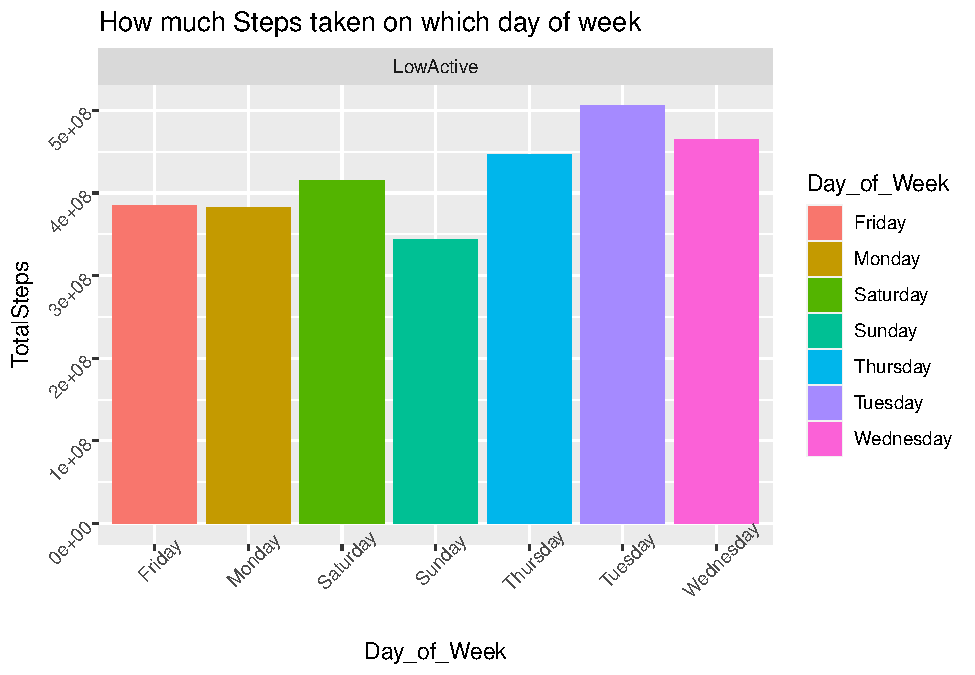
\includegraphics{markdownFile_files/figure-latex/unnamed-chunk-49-1.pdf}

\hypertarget{observations}{%
\subsection{Observations}\label{observations}}

we can see the smart device works very well on sleep data and calories
burned

\begin{Shaded}
\begin{Highlighting}[]
\FunctionTok{ggplot}\NormalTok{(}\AttributeTok{data =}\NormalTok{ Activity)}\SpecialCharTok{+}
  \FunctionTok{geom\_col}\NormalTok{(}\AttributeTok{mapping =} \FunctionTok{aes}\NormalTok{(Day\_of\_Week, }\AttributeTok{y=}\NormalTok{TotalSteps, }\AttributeTok{fill =}\NormalTok{Day\_of\_Week))}\SpecialCharTok{+}
  \FunctionTok{facet\_grid}\NormalTok{(}\SpecialCharTok{\textasciitilde{}}\NormalTok{DistanceCategory)}\SpecialCharTok{+}
  \FunctionTok{labs}\NormalTok{(}\AttributeTok{title =} \StringTok{"How much Steps taken on which day of week"}\NormalTok{)}\SpecialCharTok{+}
  \FunctionTok{theme}\NormalTok{(}\AttributeTok{axis.text =} \FunctionTok{element\_text}\NormalTok{(}\AttributeTok{angle =} \DecValTok{45}\NormalTok{))}
\end{Highlighting}
\end{Shaded}

\includegraphics{markdownFile_files/figure-latex/unnamed-chunk-50-1.pdf}

Observations\_ by data viz we can say on sunday there are less data for
totalsteps taken due to holiday on tuesday again back to routine work so
good steps are taken and on other days average steps are taken

\hypertarget{recommendations}{%
\subsection{Recommendations:}\label{recommendations}}

The app which is made must have to update to track all the data which is
needed from the smart devices.

So I would like to suggest the company must have to work on the app to
get these information consistently and accurately.

Because the smart devices are rooted to the mobile to track the
information from the consumers through the smart devices.

The age of the consumer not tracked so I would like to add the age data
to this app to get accurate results.

\hypertarget{add-new-column-totalactiveminutes-to-activity-which-is-the-sum-of-all-three-activeminutes-columns}{%
\subsubsection{2. Add new column TotalActiveMinutes to Activity which is
the sum of all three ActiveMinutes
columns:}\label{add-new-column-totalactiveminutes-to-activity-which-is-the-sum-of-all-three-activeminutes-columns}}

\begin{Shaded}
\begin{Highlighting}[]
\NormalTok{Activity }\OtherTok{\textless{}{-}}\NormalTok{ Activity }\SpecialCharTok{\%\textgreater{}\%}
  \FunctionTok{rowwise}\NormalTok{() }\SpecialCharTok{\%\textgreater{}\%}
  \FunctionTok{mutate}\NormalTok{(}\AttributeTok{TotalActiveMinutes =} \FunctionTok{sum}\NormalTok{(}\FunctionTok{c}\NormalTok{(VeryActiveMinutes, FairlyActiveMinutes, LightlyActiveMinutes)))}
\end{Highlighting}
\end{Shaded}

\hypertarget{next-i-created-new-columns-with-categories-in-datasets}{%
\subsubsection{Next, I created new columns with categories in
datasets}\label{next-i-created-new-columns-with-categories-in-datasets}}

\hypertarget{sleep_day}{%
\subsubsection{1. Sleep\_Day}\label{sleep_day}}

\begin{Shaded}
\begin{Highlighting}[]
\NormalTok{Sleep\_Day }\OtherTok{=}\NormalTok{ Sleep\_Day }\SpecialCharTok{\%\textgreater{}\%} \FunctionTok{mutate}\NormalTok{(}\AttributeTok{Sleep\_Amount =} \FunctionTok{case\_when}\NormalTok{(TotalMinutesAsleep}\SpecialCharTok{/}\DecValTok{60}\SpecialCharTok{\textgreater{}=}\FloatTok{6.0} \SpecialCharTok{\&}\NormalTok{ TotalMinutesAsleep}\SpecialCharTok{/}\DecValTok{60}\SpecialCharTok{\textless{}=}\FloatTok{9.0}   \SpecialCharTok{\textasciitilde{}} \StringTok{"Good Sleep"}\NormalTok{,}
\NormalTok{    TotalMinutesAsleep}\SpecialCharTok{/}\DecValTok{60}\SpecialCharTok{\textless{}}\FloatTok{6.0} \SpecialCharTok{\textasciitilde{}} \StringTok{"Under Sleep"}\NormalTok{, }
\NormalTok{    TotalMinutesAsleep}\SpecialCharTok{/}\DecValTok{60}\SpecialCharTok{\textgreater{}}\FloatTok{9.0} \SpecialCharTok{\textasciitilde{}} \StringTok{"Over sleep"}\NormalTok{))}
    
\NormalTok{   New\_Weight }\OtherTok{\textless{}{-}}\NormalTok{ WeightLogInfo }\SpecialCharTok{\%\textgreater{}\%}
     \FunctionTok{select}\NormalTok{(Id,Date,WeightKg,BMI)}
\end{Highlighting}
\end{Shaded}

\hypertarget{since-id-is-in-dbl-data-type-we-have-to-convert-it-into-character-type-of-all-dataframes-1}{%
\subsubsection{since Id is in dbl data type we have to convert it into
character type of all
dataframes}\label{since-id-is-in-dbl-data-type-we-have-to-convert-it-into-character-type-of-all-dataframes-1}}

\begin{Shaded}
\begin{Highlighting}[]
\NormalTok{Activity }\OtherTok{\textless{}{-}} \FunctionTok{mutate}\NormalTok{(Activity, }\AttributeTok{Id=}\FunctionTok{as.character}\NormalTok{(}\StringTok{\textquotesingle{}Id\textquotesingle{}}\NormalTok{))}
\NormalTok{Hourly\_Intensities }\OtherTok{\textless{}{-}}\FunctionTok{mutate}\NormalTok{(Hourly\_Intensities,}\AttributeTok{Id=}\FunctionTok{as.character}\NormalTok{(}\StringTok{\textquotesingle{}Id\textquotesingle{}}\NormalTok{))}
\NormalTok{Hourly\_Calories }\OtherTok{\textless{}{-}} \FunctionTok{mutate}\NormalTok{(Hourly\_Calories,}\AttributeTok{Id=}\FunctionTok{as.character}\NormalTok{(}\StringTok{\textquotesingle{}Id\textquotesingle{}}\NormalTok{))}
\NormalTok{Hourly\_Steps }\OtherTok{\textless{}{-}} \FunctionTok{mutate}\NormalTok{(Hourly\_Steps,}\AttributeTok{Id=}\FunctionTok{as.character}\NormalTok{(}\StringTok{\textquotesingle{}Id\textquotesingle{}}\NormalTok{))}
\NormalTok{Heartrate\_Seconds }\OtherTok{\textless{}{-}} \FunctionTok{mutate}\NormalTok{(Heartrate\_Seconds,}\AttributeTok{Id=}\FunctionTok{as.character}\NormalTok{(}\StringTok{\textquotesingle{}Id\textquotesingle{}}\NormalTok{))}
\NormalTok{Sleep\_Day }\OtherTok{\textless{}{-}} \FunctionTok{mutate}\NormalTok{(Sleep\_Day,}\AttributeTok{Id=}\FunctionTok{as.character}\NormalTok{(}\StringTok{\textquotesingle{}Id\textquotesingle{}}\NormalTok{))}
\NormalTok{WeightLogInfo }\OtherTok{\textless{}{-}}\FunctionTok{mutate}\NormalTok{(WeightLogInfo,}\AttributeTok{Id=}\FunctionTok{as.character}\NormalTok{(}\StringTok{\textquotesingle{}Id\textquotesingle{}}\NormalTok{))}
\end{Highlighting}
\end{Shaded}

\hypertarget{check-it-1}{%
\subsubsection{check it}\label{check-it-1}}

\begin{Shaded}
\begin{Highlighting}[]
\FunctionTok{summary}\NormalTok{(Activity)}
\end{Highlighting}
\end{Shaded}

\begin{verbatim}
##       Id             ActivityDate          TotalSteps    TotalDistance   
##  Length:385400      Min.   :2016-04-12   Min.   :    0   Min.   : 0.000  
##  Class :character   1st Qu.:2016-04-19   1st Qu.: 3790   1st Qu.: 2.620  
##  Mode  :character   Median :2016-04-26   Median : 7406   Median : 5.245  
##                     Mean   :2016-04-26   Mean   : 7638   Mean   : 5.490  
##                     3rd Qu.:2016-05-04   3rd Qu.:10727   3rd Qu.: 7.713  
##                     Max.   :2016-05-12   Max.   :36019   Max.   :28.030  
##  VeryActiveDistance ModeratelyActiveDistance LightActiveDistance
##  Min.   : 0.000     Min.   :0.0000           Min.   : 0.000     
##  1st Qu.: 0.000     1st Qu.:0.0000           1st Qu.: 1.945     
##  Median : 0.210     Median :0.2400           Median : 3.365     
##  Mean   : 1.503     Mean   :0.5675           Mean   : 3.341     
##  3rd Qu.: 2.053     3rd Qu.:0.8000           3rd Qu.: 4.782     
##  Max.   :21.920     Max.   :6.4800           Max.   :10.710     
##  VeryActiveMinutes FairlyActiveMinutes LightlyActiveMinutes SedentaryMinutes
##  Min.   :  0.00    Min.   :  0.00      Min.   :  0.0        Min.   :   0.0  
##  1st Qu.:  0.00    1st Qu.:  0.00      1st Qu.:127.0        1st Qu.: 729.8  
##  Median :  4.00    Median :  6.00      Median :199.0        Median :1057.5  
##  Mean   : 21.16    Mean   : 13.56      Mean   :192.8        Mean   : 991.2  
##  3rd Qu.: 32.00    3rd Qu.: 19.00      3rd Qu.:264.0        3rd Qu.:1229.5  
##  Max.   :210.00    Max.   :143.00      Max.   :518.0        Max.   :1440.0  
##     Calories    Day_of_Week        TotalMinutesAsleep Sleep_Amount      
##  Min.   :   0   Length:385400      Min.   : 58.0      Length:385400     
##  1st Qu.:1828   Class :character   1st Qu.:361.0      Class :character  
##  Median :2134   Mode  :character   Median :432.5      Mode  :character  
##  Mean   :2304                      Mean   :419.2                        
##  3rd Qu.:2793                      3rd Qu.:490.0                        
##  Max.   :4900                      Max.   :796.0                        
##  DistanceCategory   TotalActiveMinutes
##  Length:385400      Min.   :  0.0     
##  Class :character   1st Qu.:146.8     
##  Mode  :character   Median :247.0     
##                     Mean   :227.5     
##                     3rd Qu.:317.2     
##                     Max.   :552.0
\end{verbatim}

\begin{Shaded}
\begin{Highlighting}[]
\NormalTok{  Activity }\OtherTok{=}\NormalTok{ Activity }\SpecialCharTok{\%\textgreater{}\%} 
  \FunctionTok{mutate}\NormalTok{(}\AttributeTok{Steps\_Amount =} \FunctionTok{case\_when}\NormalTok{(TotalSteps}\SpecialCharTok{\textless{}=}\DecValTok{4500} \SpecialCharTok{\textasciitilde{}} \StringTok{"Less Walker"}\NormalTok{,}
\NormalTok{    TotalSteps}\SpecialCharTok{\textgreater{}}\DecValTok{4000} \SpecialCharTok{\&}\NormalTok{ TotalSteps }\SpecialCharTok{\textless{}=}\DecValTok{9000} \SpecialCharTok{\textasciitilde{}} \StringTok{"Good Walker"}\NormalTok{, TotalSteps}\SpecialCharTok{\textgreater{}}\DecValTok{9000} \SpecialCharTok{\&}\NormalTok{ TotalSteps}\SpecialCharTok{\textless{}=}\DecValTok{12000} \SpecialCharTok{\textasciitilde{}} \StringTok{"Better Walker"}\NormalTok{,}
\NormalTok{    TotalSteps}\SpecialCharTok{\textgreater{}}\DecValTok{12000} \SpecialCharTok{\textasciitilde{}} \StringTok{"Best Walker"}\NormalTok{))}
\end{Highlighting}
\end{Shaded}

\begin{Shaded}
\begin{Highlighting}[]
\NormalTok{New\_Weight }\OtherTok{=}\NormalTok{ New\_Weight }\SpecialCharTok{\%\textgreater{}\%} 
\FunctionTok{mutate}\NormalTok{(}\AttributeTok{Weight\_Amount =} \FunctionTok{case\_when}\NormalTok{(BMI }\SpecialCharTok{\textless{}=} \FloatTok{18.5} \SpecialCharTok{\textasciitilde{}} \StringTok{"UnderWeight"}\NormalTok{, BMI }\SpecialCharTok{\textgreater{}=} \FloatTok{18.6} \SpecialCharTok{\&}\NormalTok{ BMI }\SpecialCharTok{\textless{}=} \FloatTok{24.9} \SpecialCharTok{\textasciitilde{}} \StringTok{"NormalWeight"}\NormalTok{, BMI }\SpecialCharTok{\textgreater{}=} \DecValTok{25} \SpecialCharTok{\&}\NormalTok{ BMI }\SpecialCharTok{\textless{}=} \FloatTok{29.9} \SpecialCharTok{\textasciitilde{}} \StringTok{"OverWeight"}\NormalTok{, BMI }\SpecialCharTok{\textgreater{}=} \DecValTok{30} \SpecialCharTok{\textasciitilde{}} \StringTok{"Obesity"}\NormalTok{))}
\end{Highlighting}
\end{Shaded}

\begin{Shaded}
\begin{Highlighting}[]
\NormalTok{Heartrate\_Seconds }\OtherTok{=}\NormalTok{ Heartrate\_Seconds }\SpecialCharTok{\%\textgreater{}\%}
\FunctionTok{mutate}\NormalTok{(}\AttributeTok{Heartrate\_Amount =} \FunctionTok{case\_when}\NormalTok{(Value }\SpecialCharTok{\textless{}=} \DecValTok{80} \SpecialCharTok{\textasciitilde{}} \StringTok{"Normal B.P."}\NormalTok{, }
\NormalTok{Value }\SpecialCharTok{\textgreater{}=} \DecValTok{81} \SpecialCharTok{\textasciitilde{}} \StringTok{"High B.P."}\NormalTok{))}
\end{Highlighting}
\end{Shaded}

\begin{Shaded}
\begin{Highlighting}[]
\NormalTok{Activity }\OtherTok{=}\NormalTok{ Activity }\SpecialCharTok{\%\textgreater{}\%} \FunctionTok{mutate}\NormalTok{(}\AttributeTok{Burned\_Calories =} \FunctionTok{case\_when}\NormalTok{(Calories}\SpecialCharTok{\textless{}=}\DecValTok{1800} \SpecialCharTok{\textasciitilde{}} \StringTok{"Low"}\NormalTok{, Calories}\SpecialCharTok{\textgreater{}}\DecValTok{1800} \SpecialCharTok{\&}\NormalTok{ Calories}\SpecialCharTok{\textless{}=}\DecValTok{2200} \SpecialCharTok{\textasciitilde{}} \StringTok{"Medium"}\NormalTok{,}
\NormalTok{    Calories}\SpecialCharTok{\textgreater{}}\DecValTok{2200} \SpecialCharTok{\&}\NormalTok{ Calories}\SpecialCharTok{\textless{}=}\DecValTok{2600} \SpecialCharTok{\textasciitilde{}} \StringTok{"High"}\NormalTok{, Calories}\SpecialCharTok{\textgreater{}}\DecValTok{2600} \SpecialCharTok{\textasciitilde{}} \StringTok{"Very High"}\NormalTok{))}
\end{Highlighting}
\end{Shaded}

\hypertarget{sedentary-time}{%
\subsubsection{4. Sedentary Time}\label{sedentary-time}}

\begin{Shaded}
\begin{Highlighting}[]
\NormalTok{Activity }\OtherTok{=}\NormalTok{ Activity }\SpecialCharTok{\%\textgreater{}\%} 
  \FunctionTok{mutate}\NormalTok{(}\AttributeTok{Sedentary\_Time =} \FunctionTok{case\_when}\NormalTok{(SedentaryMinutes  }\SpecialCharTok{\textgreater{}} \DecValTok{626} \SpecialCharTok{\textasciitilde{}} \StringTok{"Good"}\NormalTok{,}
\NormalTok{    SedentaryMinutes }\SpecialCharTok{\textless{}} \DecValTok{627} \SpecialCharTok{\&}\NormalTok{ SedentaryMinutes  }\SpecialCharTok{\textasciitilde{}} \StringTok{"Good"}\NormalTok{, SedentaryMinutes}\SpecialCharTok{/}\DecValTok{60}\SpecialCharTok{\textgreater{}}\DecValTok{10} \SpecialCharTok{\&}\NormalTok{ SedentaryMinutes}\SpecialCharTok{/}\DecValTok{60}\SpecialCharTok{\textless{}=}\DecValTok{12} \SpecialCharTok{\textasciitilde{}} \StringTok{"Bad"}\NormalTok{,}
\NormalTok{    SedentaryMinutes}\SpecialCharTok{/}\DecValTok{60}\SpecialCharTok{\textgreater{}}\DecValTok{12} \SpecialCharTok{\textasciitilde{}} \StringTok{"Very Bad"}\NormalTok{))}
\end{Highlighting}
\end{Shaded}

\hypertarget{changing-data-type-of-date-column-1}{%
\subsubsection{changing data type of date
column}\label{changing-data-type-of-date-column-1}}

\hypertarget{hourly_calories}{%
\subsubsection{Hourly\_Calories}\label{hourly_calories}}

\begin{Shaded}
\begin{Highlighting}[]
\NormalTok{Hourly\_Calories}\SpecialCharTok{$}\NormalTok{ActivityHour}\OtherTok{=}\FunctionTok{as.POSIXct}\NormalTok{(Hourly\_Calories}\SpecialCharTok{$}\NormalTok{ActivityHour, }\AttributeTok{format=}\StringTok{"\%m/\%d/\%Y \%I:\%M:\%S \%p"}\NormalTok{, }\AttributeTok{tz=}\FunctionTok{Sys.timezone}\NormalTok{())}
\NormalTok{Hourly\_Calories}\SpecialCharTok{$}\NormalTok{ActivityHour }\OtherTok{\textless{}{-}} \FunctionTok{format}\NormalTok{(Hourly\_Calories}\SpecialCharTok{$}\NormalTok{ActivityHour, }\AttributeTok{format =} \StringTok{"\%m/\%d/\%y"}\NormalTok{)}
\end{Highlighting}
\end{Shaded}

\hypertarget{heartrate_seconds}{%
\subsubsection{Heartrate\_Seconds}\label{heartrate_seconds}}

\begin{Shaded}
\begin{Highlighting}[]
\NormalTok{Heartrate\_Seconds}\SpecialCharTok{$}\NormalTok{Time}\OtherTok{=}\FunctionTok{as.POSIXct}\NormalTok{(Heartrate\_Seconds}\SpecialCharTok{$}\NormalTok{Time, }\AttributeTok{format=}\StringTok{"\%m/\%d/\%Y \%I:\%M:\%S \%p"}\NormalTok{, }\AttributeTok{tz=}\FunctionTok{Sys.timezone}\NormalTok{())}
\NormalTok{Heartrate\_Seconds}\SpecialCharTok{$}\NormalTok{Time }\OtherTok{\textless{}{-}} \FunctionTok{format}\NormalTok{(Heartrate\_Seconds}\SpecialCharTok{$}\NormalTok{Time, }\AttributeTok{format =} \StringTok{"\%m/\%d/\%y"}\NormalTok{)}
\end{Highlighting}
\end{Shaded}

\hypertarget{weightloginfo}{%
\subsubsection{WeightLogInfo}\label{weightloginfo}}

\begin{Shaded}
\begin{Highlighting}[]
\NormalTok{WeightLogInfo}\SpecialCharTok{$}\NormalTok{Date}\OtherTok{=}\FunctionTok{as.POSIXct}\NormalTok{(WeightLogInfo}\SpecialCharTok{$}\NormalTok{Date, }\AttributeTok{format=}\StringTok{"\%m/\%d/\%Y \%I:\%M:\%S \%p"}\NormalTok{, }\AttributeTok{tz=}\FunctionTok{Sys.timezone}\NormalTok{())}
\NormalTok{WeightLogInfo}\SpecialCharTok{$}\NormalTok{Date }\OtherTok{\textless{}{-}} \FunctionTok{format}\NormalTok{(WeightLogInfo}\SpecialCharTok{$}\NormalTok{Date, }\AttributeTok{format =} \StringTok{"\%m/\%d/\%y"}\NormalTok{)}
\end{Highlighting}
\end{Shaded}

\hypertarget{hourly_intensities}{%
\subsubsection{hourly\_Intensities}\label{hourly_intensities}}

\begin{Shaded}
\begin{Highlighting}[]
\NormalTok{Hourly\_Intensities}\SpecialCharTok{$}\NormalTok{ActivityHour}\OtherTok{=}\FunctionTok{as.POSIXct}\NormalTok{(Hourly\_Intensities}\SpecialCharTok{$}\NormalTok{ActivityHour, }\AttributeTok{format=}\StringTok{"\%m/\%d/\%Y \%I:\%M:\%S \%p"}\NormalTok{, }\AttributeTok{tz=}\FunctionTok{Sys.timezone}\NormalTok{())}
\NormalTok{Hourly\_Intensities}\SpecialCharTok{$}\NormalTok{ActivityHour }\OtherTok{\textless{}{-}} \FunctionTok{format}\NormalTok{(Hourly\_Intensities}\SpecialCharTok{$}\NormalTok{ActivityHour, }\AttributeTok{format =} \StringTok{"\%H:\%M:\%S"}\NormalTok{)}
\NormalTok{Hourly\_Intensities}\SpecialCharTok{$}\NormalTok{ActivityHour }\OtherTok{\textless{}{-}} \FunctionTok{format}\NormalTok{(Hourly\_Intensities}\SpecialCharTok{$}\NormalTok{ActivityHour, }\AttributeTok{format =} \StringTok{"\%m/\%d/\%y"}\NormalTok{)}
\end{Highlighting}
\end{Shaded}

\hypertarget{recommendations-1}{%
\subsubsection{Recommendations:}\label{recommendations-1}}

The app which is made must have to update to track all the data which is
needed from the smart devices.

So I would like to suggest the company must have to work on the app to
get these information consistently and accurately.

Because the smart devices are rooted to the mobile to track the
information from the consumers through the smart devices.

The age of the consumer not tracked so I would like to add the age data
to this app to get accurate results.

\end{document}
